%
% Documento: Referencial Teórico
%

\chapter{Mobilidade Urbana em Cidades Inteligentes}\label{chap:Mobilidade Urbana em Cidades Inteligentes} %referencial teórico  

\begin{comment}
\mnote{Patrícia: Esse capítulo ainda tá um pouco confuso. As seções e subseções tem que conversar. Ainda parece um monte de coisa costurada. A ideia é começar a falar de Cidades Inteligentes e quando falar disso pega o que falamos naquela artigo, sobre a infraestrutura necessária e aí sim vc pode falar de computação e nuvem e PaaS, IaaS e SaaS. 
Na continuação sobre cidades inteligentes vc vai falar mais detalhadamente sobre mobilidade inteligente que é uma das dimensões que aquele autor propõe. Da uma olhada naquele artigo que a ideia eh aquela.
Quando vc falar de mobilidade vc insere o conceito de MaaS e somente depois de tudo isso vc falar sobre campus inteligente. 

Acho que nao cabe aqui ainda falar sobre carona solidária pq seu projeto mudou um pouco o foco devido todos os problemas. Vc vai falar de carona solidária somente na outra seção, quando for apresentar as soluções de mobilidade que foram encontradas, fará o comparativo e chegará na carona solidária.}

\end{comment}

\section{Computação em Nuvem}
A Computação em Nuvem (\textit{Cloud Computing}) vem causando muitas transformações digitais e já tem um lugar de destaque nas CI. Embora atualmente seja algo bastante usual, esse é um assunto grande e complexo que possui vários subtemas, como os modelos de nuvem.

Dentro da Computação em nuvem é comum encontrarmos três modelos de disponibilização de serviços: 

Infraestrutura como serviço, oferece acesso baseado na web para armazenamento e poder de computação. O consumidor não precisa gerenciar ou controlar a subjacente infraestrutura em nuvem, mas tem controle sobre os sistemas operacionais, armazenamento, e aplicativos implantados.

Plataforma como serviço, onde os usuários hospedam um
ambiente para suas aplicações. Os usuários controlam os aplicativos, mas não controlam o sistema operacional, hardware ou infraestrutura de rede que são usados.

Software como serviço, é onde o consumidor usa um aplicativo, mas não controla o funcionamento do sistema, hardware ou infraestrutura de rede. Nesta situação, o usuário orienta os aplicativos pela rede. 

\citeonline{infra-cloud} diz que os serviços oferecidos pela Computação em Nuvem são semelhantes ao serviço de energia elétrica, pagamos apenas o que consumimos. Por consequência, necessidades como as de investir em equipamentos e infraestruturas de TIC são reduzidos.
% permitindo que seus usuários se conectem globalmente sem precisar implementar infraestruturas locais.

%consideravelmente, permitindo que seus usuários se conectem e façam colaborações globalmente sem configurar
%infraestruturas, como servidores, e com uma alta escalabilidade e capacidade de acomodar inúmeros usuários. 

%que seus usuários se conectem globalmente sem precisarem configurar infraestruturas de TI locais.

Vale ressaltar que a capacidade de uma CI ser dinâmica e automática faz ela precisar de infraestruturas robustas e capazes de suprir as necessidades de estar todo tempo online, algo que a computação em nuvem consegue oferecer através de serviços altamente disponíveis, elásticos, flexíveis e robustos. \cite{kon-cloud}.



%A imagem abaixo descreve bem as responsabilidades de cada camada da cloud:

\begin{comment}

\begin{figure}[!hbtp]
\centering
\caption{Camadas de Nuvem e suas responsabiidades.}
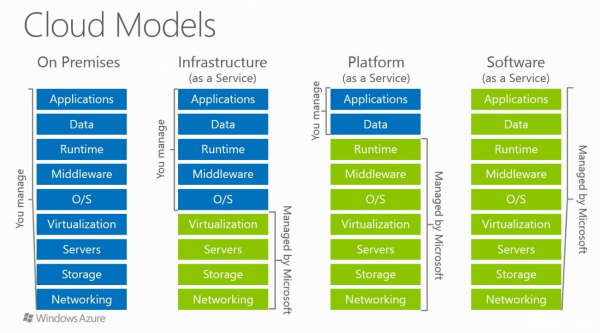
\includegraphics[width=8cm]{./04-figuras/azure-cloud.png}
\label{cloud-computing}
\fonte{https://www.lambda3.com.br/2017/08/iaas-paas-e-saas-qual-a-diferenca/}
\end{figure}
	conteúdo...
\end{comment}



\section{Cidades Inteligentes}

Cidades Digitais, CI, são cidades que utilizam um ambiente inovador caracterizado pela utilização de TIC. Segundo \citeonline{yin} os termos se referem a ação de utilizar a tecnologia em favor da melhoria da qualidade de vida, do gerenciamento de recursos e da infraestrutura das cidades.

Estas cidades sempre buscam otimizar recursos para melhor atender as necessidades dos cidadãos, interconectando informações, gerenciando operações sempre envolvendo uma infraestrutura tecnológica, sistemas inovadores e colaboração digital. \cite{washburn2010helping}.

% isso vale para mobilidade, para o setor imobiliário, saúde e entre outros serviços que de alguma forma podem ser otimizados usando TIC’s \cite{washburn2010helping}.

Já \citeonline{giffinger} acrescentam características para serem considerados antes de desenvolver uma CI. Para os autores, deve ser avaliado um todo, como consciência, flexibilidade, transformabilidade, individualidade, e comportamento estratégico da cidade e de seus cidadãos, e destaca que todos precisam ter conhecimento da posição da cidade e o que precisa ser feito para alcançar o status de CI. 

Segundo \citeonline{neirotti}, TIC não definem uma CI, são apenas uma das soluções utilizadas. O autor ainda explica que as cidades mais equipadas não implicam necessariamente nas melhores CI e o número de iniciativas não indicam performance, apenas demonstra o número de esforços para melhorar a vida dos cidadãos. 


\begin{comment}

De acordo com \citeonline{dameri}: 
\begin{citacao}
“Uma Cidade Inteligente é uma área geográfica bem definida, na qual altas tecnologias, como TIC, logística, produção de energia, etc., cooperam para criar benefícios para os cidadãos em termos de bem-estar, inclusão e participação, qualidade ambiental, desenvolvimento inteligente; é governado por um conjunto bem definido de assuntos, capaz de declarar as regras e políticas para o governo e o desenvolvimento da cidade”. (tradução nossa)."
%\footnote{Texto original: "A smart city is a well-defined geographical area, in which high technologies such as ICT, logistic, energy production, and so on, cooperate to create benefits for citizens in terms of well-being, inclusion and participation, environmental quality, intelligent development ; it is governed by a well-defined pool of subjects, able to state the rules and policy for the city government and development."}
\end{citacao}
\end{comment} 

CI em estudos de \citeonline{giffinger}, citado  por \citeonline{kon}, apresenta uma forma de como as cidades ditas inteligentes podem ser mensuradas e avaliadas, o mesmo cita 6 dimensões que possuem suas características próprias. Na Tabela \ref{tab:tabela1} veremos quais são:

% Please add the following required packages to your document preamble:
% \usepackage[table,xcdraw]{xcolor}
% If you use beamer only pass "xcolor=table" option, i.e. \documentclass[xcolor=table]{beamer}

\begin{table}[h]
\centering
\caption{Aspectos de Cidades Inteligentes}
\label{tab:tabela1}
\vspace{0.0cm}
\begin{tabular}{cp{10cm}}
\hline
 & Definição \\
\hline
\vspace{0.05cm}
Economia Inteligente & 
É a competitividade econômica, empreendedorismo, produtividade, leis que ajudem a inovar e incentivar a criação de novas soluções tecnológicas. \\
\hline
\vspace{0.05cm}
População Inteligente & 
Mede a qualidade da educação da população, seus postos de trabalho e renda, além de avaliar a interação social, os incentivos a programas de educação e incentivos a produção científica e tecnológica. \\
\hline
\vspace{0.05cm}
Governança Inteligente & Avalia o quão transparente e participativo é o governo por meio de seus portais, como são feitas as tomadas de decisões e serviços públicos e sociais.\\
\hline
\vspace{0.05cm}
Mobilidade Inteligente & Trata-se das questões de acessibilidade e mobilidade local onde se leva em consideração os congestionamentos, os transportes utilizados, o uso de combustível fóssil e as soluções tecnológicas que são utilizadas para melhorar o transporte da população.
% sempre priorizando os que menos prejudicam o meio ambiente e o fluxo urbano das cidades.
 \\
\hline
\vspace{0.05cm}
Ambiente Inteligente &
É avaliado quais soluções as cidades possuem para degradar menos o meio ambiente e quais recursos são reaproveitados, como água, energia, lixo.
% energia renovável, lixo reciclado e etc. 
\\
\hline
Vida Inteligente &
A qualidade de vida voltada para a segurança da cidade, da saúde das pessoas, o lazer, qualidade na moradia, serviços culturais.
%Este projeto tem como foco trabalhar apenas na mobilidade inteligente, que por meio de soluções tecnológicas tem melhorado bastante o fluxo nas ruas e estradas brasileiras.

\end{tabular}
\end{table}


\begin{comment}
	Contudo, CI não tem uma definição formal amplamente aceita, embora haja muitos conceitos sobre o tema, Cidade Digital é o que mais se destaca. Alguns autores abordam a diferença entre cidades inteligentes e cidades digitais.
	
	%%Sintetizar este paragrafo, muito grande
	%Segundo  \citeonline{yin}, 
	Cidades digitais se refere a digitalização de uma cidade, envolvendo informações, acesso ao dados e visualizações por parte da população, a cidade digital está mais ligada na forma em que a cidade utiliza e se moderniza com a combinação de comunicação e infraestrutura computacional para fornecer as informações públicas, já cidades inteligentes é uma definição que pode ser considerada como a junção do entendimento de cidade digital e sociedade do conhecimento, onde as pessoas envolvidas são responsáveis pelo aprimoramento do local criando zonas de colaboração digital \cite{yin}.
	%“o objetivo de uma cidade inteligente é transformar a vida e o trabalho dentro de uma região de maneira significativa e fundamental, não incremental” \cite{yin} (tradução nossa).
\end{comment}


Quando se fala a respeito do gerenciamento dos projetos de CI, \citeonline{chourabi} indicam que uma característica comum das iniciativas são que a maioria das cidades inteligentes são gerenciadas e organizadas por governos e utilizam o uso massivo de TIC. 

Uma iniciativa realizada no Brasil, até mencionada por \citeonline{namepardo}, é a da cidade de Porto Alegre, reconhecida nacionalmente e internacionalmente, a cidade tem tomado medidas usando tecnologia para o auxílio desde 2006 quando decidiu investir pesado na implementação de uma rede de fibra ótica para os serviços do governo , garantindo mais de 99.8 \% de disponibilidade \cite{weiss}.

 São Paulo se destaca também como o maior centro de pesquisa sobre o tema com muitas publicações e diversos trabalhos relacionados às áreas envolvidas, tendo a USP entre os destaques no número de publicações \cite{lazzaretti}. 


E para alcançarmos um nível de CI, algumas coisas precisam ser pensadas antes. Soluções que auxiliem questões como segurança, saúde, educação, ou mesmo lazer são fundamentais. Ações desde a construção de áreas verdes, de centros de cultura e monitoramento da cidade utilizando câmeras e mapeamento de zonas pouco seguras são essenciais. 

No entanto, a população não irá usufruir de nenhuma das soluções desenvolvidas para quaisquer das dimensões apontadas se não acontecer uma inclusão tecnológica massiva com programas de incentivo à educação científica e tecnológica. Caso contrário, parte da população será excluída e segregada da cidade \cite{patricia}.

Além disso, para construir uma CI fatores importantes como inclusão digital e infraestrutura tecnológica precisam ser discutidos. Para que estás soluções funcionem de maneira efetiva é necessário que elas sejam desenvolvidas considerando um sistema de computação que tenha uma arquitetura heterogênea e distribuída. As arquiteturas mais utilizadas atualmente são as em nuvem, devido sua capacidade de suportar grande demanda e a escalabilidade \cite{patricia}. 

\begin{comment}
	A arquitetura se dá primeiramente através de dispositivos de borda que são responsáveis por coletar dados dos dispositivos de internet da coisas espalhados pelo ambiente, a característica desses dispositivos é de serem de baixo processamento e capacidade. Após o processo de coleta, os dispositivos de borda enviam os dados para a nuvem para serem processados e armazenados. A rede tem características homogêneas com extrema importância de serem altamente disponíveis e capazes de oferecer acesso de milhares de pessoas por meio de seus dispositivos. Mais uma vantagem da computação em nuvem é se tratando de valores, segundo \cite{patricia}, a contratação de serviços em nuvem diminui os altos gastos em infraestrutura, a contratação conforme as necessidades das aplicações trazem uma grande vantagem, economia que não cria problema para os usuários, os serviços de nuvem oferecidos devolvem o resultado esperado.
\end{comment}


\section{Mobilidade Inteligente}
%\mnote{compartilhamento de carros}
%\mnote{compartilhamento de viagens}
%\mnote{transporte sob demanda}
%\mnote{Falar sobre as tecnologias que tornam possível a utilização de ferramentas de mobilidade inteligente; gps, smartphones, cloud}
%Com o passar dos anos, A mobilidade urbana está necessitando cada vez mais de atenção. 

%Com o aumento do número de pessoas e veículos surgem alguns problemas  como engarrafamentos cada vez maiores, dificuldade de locomoção de pedestres e ciclistas, poluição do ar. 

%No entanto, \citeonline{santana} diz que a Mobilidade Urbana vai além de trânsito lento e grandes congestionamentos, a mobilidade urbana carrega a importância da cidadania de um povo.

\citeonline{giffinger} afirma que mobilidade inteligente trata-se de acessibilidade nacional e internacional dando importância as tecnologias modernas advindas da TICs e sistemas de transporte sustentáveis. O uso de uma tecnologia moderna que de suporte a mobilidade faz surgir sistemas "inteligentes".

Além disso, otimizar a logística dentro de áreas urbanas, fornecer aos cidadãos um sistema dinâmico e multimodal, assegurar um transporte sustentável e ecológico e ainda levar em consideração as condições de tráfego e energia melhoram o transito urbano e mobilidade dos habitantes \cite{neirotti}. %\cite{giffinger}.

Modais como ônibus, metros, carros e bicicletas são avaliados em relação a sua facilidade de mobilidade. Analisar o tamanho da malha viária, ciclovias, uso de transporte poluentes e não poluentes, uso de transporte público também são parâmetros considerados \cite{kon}. 

Muitas iniciativas começaram a criar soluções tecnológicas com objetivos de tratar essas "dores" \cite{cocchia}. Dois projetos na cidade de Mdadrid (Espanha) que utilizam os celulares dos cidadãos, um de monitoramento em tempo real da posição do transporte publico e outro informando estimando a lotação dos coletivos são dignos de nota.

Hoje em dia é possível monitorar todo e qualquer tipo de transporte, o GPS é um dos dispositivos que nos auxiliam nisso. Na cidade de São Paulo, a Startup Scipopulis monitora em tempo real 14 mil ônibus obtendo dados da velocidade média das vias, acidentes ocorridos naquele momento, a quantidade de ônibus transitando na mesma via. Todos essas informações são passadas para a companhia da transporte da cidade para possíveis melhorias na mobilidade da cidade de São Paulo \cite{kon}.


%Diante do exposto, a Mobilidade Urbana

%Das várias iniciativas de cidades inteligentes, a mobilidade tem um lugar de destaque por apresentar várias soluções que já apresentam uma melhora no trajeto das pessoas em várias cidades utilizando TIC. 



% a exemplo disso, aplicativos como Uber, 99 circulam pelas cidades utilizando a mobilidade como um serviço.

%Aplicativos de carona como o BlaBlaCar  que a relação entre o motorista e o passageiro fica a critério do motorista em relação aos custos da viagem. Estas ferramentas já contribuem com a melhoria da mobilidade sem a necessidade de investimento público. 

%Uma mudança que estas aplicações apresentam é a de lugares ocupados dentro de um mesmo veículo. Segundo pesquisa realizada pela BlablaCar em 2018, a taxa de ocupação de pessoas usando o aplicativo por veículo no Brasil é de 3,8 incluindo o motorista, contra 1,9 pessoas por veículo sem o uso de do aplicativo, na mesma pesquisa, a empresa apresenta dados que as caronas solidárias ajudam na economia de CO² alegando que pessoas que  fazem o mesmo trajeto todo dia e possuem carros podem participar de um rodízio de caronas, por exemplo, nesta conta, teríamos todo dia 1 carro a menos nas ruas.

%Hoje em dia são algumas dessas soluções, aplicativos como BlaBlaCar, outros aplicativos de carona solidária mobilizado por universidades como o Caronaê da UFRJ\footnote{Disponível em: https://caronae.org/. Acesso em: 23 Jun. 2020.}, entre outras,  que movimentam o conceito de mobilidade urbana inteligente no país.

%1 - O que é?

%2 - A mobildade urbana e inteligente

%3 - A importancia da mobilidade inteligente

% serviços já existentes (uber, 99, falar um pouco de maas); mobilidade como serviço
% carona solidária

%Cocchia (2014) -a adoção de políticas de crescimento requer que as cidades
%passem a buscar projetos com o fornecimento de soluções para mobilidade urbana. As cidades
%inteligentes incialmente eram chamadas de cidades digitais por incorporar ao seu conceito
%apenas o uso de tecnologia da informação. Com a evolução passaram a incluir os conceitos de
%sustentabilidade aos seus projetos. A mobilidade urbana em cidades inteligentes faz surgir o
%5conceito da “mobilidade urbana inteligente”.

\section{Campus Inteligente}

Um campus inteligente é o reflexo de uma cidade em uma escala menor, nos campos temos relações sociais, relações administrativas, meio ambiente, serviços de coleta, mobilidade, alimentação, energia, entre outros.

Conforme \citeonline{zhang}, o comportamento de uma Campus Universitário Inteligente é semelhante ao de uma CI, porém, com um número de problemas menores, e de proporções menores, onde pode ocorrer roubos, acidentes de carro, circulação de pessoas em lugares proibidos ou outras situações não permitidas \cite{garay2018}.

Assim como cidades inteligentes, campus inteligente ou universidade inteligente não tem um conceito totalmente definido, \citeonline{alghamdi} explica que o campus inteligente surge da necessidade de oferecer serviços de alta qualidade reduzindo custos, e que isso não fica apenas nos aspectos acadêmicos, mas envolve aspectos sociais, meio ambiente, e financeiros da Universidade.

\begin{comment}
Na Figura \ref{alghamdi}, temos:
\begin{figure}[!hbtp]
\centering
\caption{Conceito de Campus Inteligente, seu impactos e suas aplicações.}
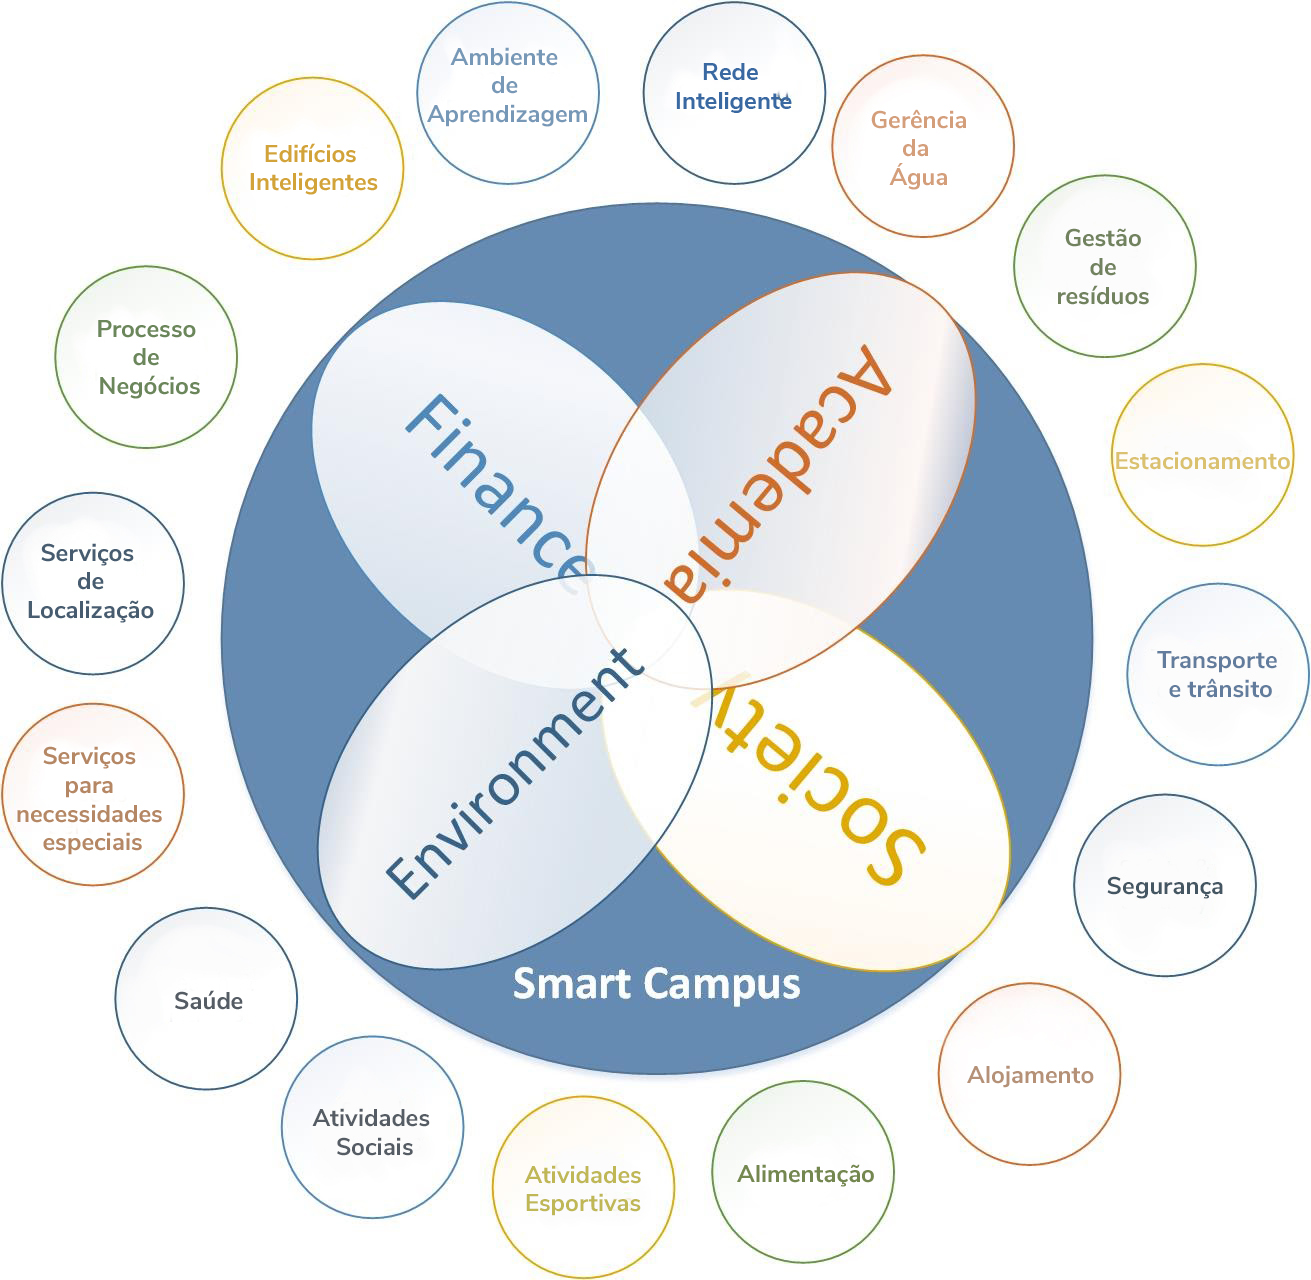
\includegraphics[width=8cm]{./04-figuras/alghamdi-edited.jpg}
\label{alghamdi}
\fonte{Adaptado de \citeonline{alghamdi}}
\end{figure}
\end{comment}




Além do conceitos e objetivos, o Campus Inteligente também tem problemas e dificuldades que o mercado impõe. \cite{alghamdi} cita 3 obstáculos: Técnico, Financeiro e Político. Semelhante as Cidades Inteligentes, deve-se considerar que ao estabelecer serviços tecnológicos a uma população, que seja de uma cidade, ou de uma universidade, conceitos de segurança, proteção e privacidade, interoperabilidade, padronização e configurações precisam estar bem encaixados para promover segurança ao uso por pessoas do Campus/Cidade, e reunir esses requisitos num ambiente tão heterogêneo, de comunicação intensiva é uma tarefa difícil \cite{alghamdi}. 

Do lado financeiro, conseguir dinheiro para levar adiante projetos que necessitam de investimentos algumas vezes elevados e experiências imaturas, ou até mesmo, sem experiência alguma com Campus Inteligente acaba dificultando iniciativas ao redor do mundo . Finalmente, os obstáculos políticos em um ambiente universitário
não são tão difíceis quanto as técnicas e financeiras devido ao
fato de que o presidente de uma universidade pode resolver a tomada de decisão processo em muitos casos; no entanto, a colaboração entre
diferentes faculdades e departamentos, reengenharia de negócios
processos e oposição de funcionários anti-tecnologia são potenciais
obstáculos que precisam ser resolvidos \cite{alghamdi}.

Por outro lado, as iniciativas tecnológicas abrem portas para recrutarmos pesquisadores, investigarmos mais sobre o tema e promover serviços e soluções inovadoras, segundo \cite{alghamdi}, a maioria dos trabalhos focados em Campus Inteligentes são sobre energia, meio ambiente e prédios inteligentes, e alguns serviços importantes, como transporte, alimentação, controle de tráfego ficam deixadas de lado.

\section{Mobilidade com Serviço - MaaS}

Mobilidade como um serviço (Mobility as a Service) é um termo utilizado para nomear uma nova tendência na mobilidade inteligente, onde empresas, organizações investem no transporte público oferecendo meios multimodais de locomoção  para a população. Algumas das características de plataformas MaaS é a facilidade de acesso, a ferramenta apresenta as opções que o usuário pode escolher para seu trajeto, facilidade no pagamento, sistema de reserva de viagens e informação em tempo real.

Sem uma definição exata, o MaaS é definido por alguns autores como a oferta de serviços de mobilidade centralizados em uma única plataforma digital, focando exclusivamente nas necessidades individuais dos usuários, sendo estes, táxis, transporte público coletivo, carros particulares, bicicletas, entre outros \cite{jittrapirom, kamargianni, mulley}.

Para não aprofundar, o objetivo da MaaS é incentivar o uso de transportes compartilhados e que seja possível o usuário planejar o seu trajeto em cima de várias opções multimodais, sejam elas, compartilhamento de carros, caronas, compartilhamentos de bicicletas, aluguel de carros, transporte público, entre outros meios de mobilidade \cite{jittrapirom}. 

\begin{comment}




\subsection{Carona Solidária}

No dicionário online define-se Carona como uma viagem sem custos para o passageiro, onde a pessoa vai pro mesmo ou para um destino próximo do destino do motorista \cite{carona}.

Carona solidária ou Carpooling consistem em compartilhar um veículo entre vários passageiros durante um trajeto para ir ao trabalho, ir a escola, a universidade, ou qualquer outro trajeto em que o ponto final seja definido. O carpooling tem ganhado mais notoriedade quando se torna um amigável e mais barato meio de transporte \cite{aissaoui}.

A carona solidária é uma prática que vem sendo utilizado por várias empresas, sejam públicas ou privadas com o objetivo de aproximar seus empregados, estreitar laços criando relações de confiança, compartilhar conhecimento e tornar os profissionais mais colaborativos \cite{oliveira2013educaccao, arasaki}. A carona solidária tende a criar relações de maneira mais amigável, assim, as pessoas tendem a conversar mais, compartilham experiências, problemas \cite{oliveira2013educaccao}.

Ainda sobre caronas solidárias, as iniciativas de carona solidária estão sendo implementadas por muitas universidades com a intenção de melhorar o acesso à instituição, sendo abordada sempre com a utilização de aplicativos e como uma medida de mobilidade inteligente e mobilidade colaborativa \cite{figueira2015mobilidade}.

Além disso,  a prática da carona solidária é vista como uma medida que impulsiona o desenvolvimento da mobilidade sustentável, onde carros antes ocupados por apenas uma pessoa será ocupado por outras, podendo haver um revezamento de carona entre os motoristas que realizam o mesmo trajeto todos os dias, sendo assim, vamos ter menos carros, logo menos poluição \cite{silveira,carpooling2013, arasaki}.



\section{Consumo Colaborativo}

Consumo colaborativo, economia colaborativa ou economia compartilhada são termos que se referem ao uso compartilhado de bens e produtos entre proprietário e cliente, o consumo colaborativo não exigem que o cliente adquira o produto, apenas “alugue”, neste novo modelo de consumo, o proprietário pode “vender” o produto por diversas vezes.

Com esse novo modelo, muitos serviços que antes funcionavam de uma forma estão mudando, a exemplo, consumo de carros, apartamentos, equipamentos, tempos e habilidades \cite{bardhi2012access}. Ebay\footnote{Disponível em: https://www.ebay.com/. Acesso em: 11 de Jul. de 2020.} (comércio eletrônico), ZipCar\footnote{Disponível em: https://www.zipcar.com/. Acesso em: 11 de Jul. de 2020.} (aluguel de carros), Freecycle\footnote{Disponível em: https://www.freecycle.com.br/. Acesso em: 11 de Jul. de 2020.} (rede de trocas de bens e serviços), iniciativas de Crowndfounding\footnote{Disponível em: https://conceitos.com/crowdfunding/. Acesso em: 13 de Jul. de 2020.} e espaços de Cowork, são ferramentas voltadas para o consumo colaborativo, cada uma em seu mercado específico \cite{santospereira}.

Diante disso, \cite{mendes2015economia} explica que a economia compartilhada vem mudando a principal característica do capitalismo mundial, onde a aquisição de bens por parte do comprador é dispensável, existindo apenas uma troca, uma facilidade de acesso ao produto sem necessidade de posse, uma relação de necessidade e posses.

Segundo \cite{bostman2011s}, o consumo colaborativo reflete sobre 3 tipos diferentes: 

\subsection{Sistema de Serviços de Produto (SSP)}

Permite compartilhar vários produtos de uma empresa (carros, filmes, objetos, acessórios), um melhor exemplo de um SSP são os casos de Netflix, Spotify, ambos oferecem os seus serviços e gerenciam direitos digitais. No Brasil várias startups trabalham nesse tipo de consumo, compartilhando bicicletas, patinetes, carros, bolsas \cite{santospereira}.


\subsection{Mercado de Redistribuição}

O mercado de redistribuição está ligado a forma de como lidamos com coisas que não nos servem mais, o passando adiante sem desperdiçá-lo, jogá-lo fora, em vez disso, mudando ele de um lugar que não é útil para um lugar que terá utilidade, esse tipo de consumo colaborativo é baseado nos princípios “reduza, reuse, recicle, recupere e redistribua” (APRENDA INVESTIMENTOS, 2016). 

\subsection{Vida Colaborativa}

Como \cite{bostman2011s} definem que a vida colaborativa é o estilo de vida onde pessoas compartilham coisas intangíveis, como seu tempo, espaço e habilidades, espaços de coworking ou pessoas que buscam outras pessoas para compartilhar conhecimento através de ferramentas também são exemplos disso.

\end{comment}